\documentclass{article}
\usepackage{ctex}
\usepackage{amsmath}
\usepackage[ruled]{algorithm2e}
\usepackage{graphicx}
\graphicspath{{pic/}}
\title{支持向量机}
\author{W.J.Z}
\date{}

\begin{document}
	\maketitle
	\section{硬间隔支持向量机}
	硬间隔指超平面能完全正确将数据划分为两类,法向量一侧为正类,相反一侧为负类,所有样本点都能满足函数间隔大于等于1的约束条件。超平面公式为:
	\begin{equation}
		w\cdot x+ b = 0
	\end{equation}
	$w$为支持向量,$b$为位移项。
	
	空间任意一点到超平面的距离为:
	\begin{equation}
	\frac{\left | w\cdot x + b \right |}{\left \| w \right \|}
	\end{equation}
	对于完全正确分类的样本,令:
	\begin{align}
	\begin{cases}
	w\cdot x_{i} + b \geq +1,& y_{i}= +1 \\
	w\cdot x_{i} + b \leq -1,& y_{i}= -1 
	\end{cases}
	\end{align}                                                                                                    两个离超平面最近的两个异类点相减得
	\begin{equation}
	w\cdot \left ( x_{1}-x_{2} \right )=\left \| w \right \|\cdot \left \| x_{1}-x_{2} \right \|\cdot \cos \theta =2
	\end{equation}                                                                                                $w \quad (x_{1}-x_{2})$为向量相乘,$\theta$为两向量之间的夹角,而$\left \| x_{1}-x_{2} \right \|\cdot \cos \theta$就是我们所求的间隔。令$d=\left \| x_{1}-x_{2} \right \|\cdot \cos \theta$,则
	\begin{equation}
	d = \frac{2}{\left \| w \right \|}
	\end{equation}     
	原始问题可描述为:
	\begin{equation}
	\mathop{max}_{w,b}\frac{2}{\left \| w \right \|}
	\label{6}
	\end{equation}                       
	\begin{equation}
	s.t. \quad  y_{i}\left ( w\cdot x_{i}+b \right )\geq 1 , \quad i=1,2,\ldots,m
	\end{equation}   
	最大化$\frac{1}{\left \| w \right \|}$等价于最小化$\left \| w \right \|^{2}$,公式\ref{6}又可描述为
	\begin{equation}
	\mathop{min}_{w,b}\frac{1}{2}\left \| w \right \|^2
	\end{equation}                 
	$$	s.t. \quad  y_{i}\left ( w\cdot x_{i}+b \right )\geq 1 , \quad i=1,2,\ldots,m$$
	引入拉格朗日乘子进行对偶化:
	\begin{equation}
	L\left ( w,b,\alpha  \right )=\frac{1}{2}\left \| w \right \|^{2}-\sum_{i=1}^{N}\alpha _{i}y_{i}\left ( w\cdot x_{i}+b \right )+\sum_{i=1}^{N}\alpha _{i}
	\label{9}
	\end{equation}
	对$w$和$b$求偏导并令其等于0得:
	\begin{equation}
	w=\sum_{i=1}^{N}\alpha _{i}y_{i}x_{i}
	\label{10}
	\end{equation}
	\begin{equation}
	\sum_{i=1}^{N}\alpha _{i}y_{i}=0
	\label{11}
	\end{equation}
	将公式\ref{10}代入公式\ref{9}和利用公式\ref{11}得:
	\begin{equation}
	\mathop{max}_{\alpha }-\frac{1}{2}\sum_{i=1}^{N}\sum_{j=1}^{N}\alpha _{i}\alpha _{j}y_{i}y_{j}\left ( x_{i}\cdot x_{j} \right ) + \sum_{i=1}^{N}\alpha _{i}
	\end{equation}
	\begin{equation}
	s.t. \quad \sum_{i=1}^{N}\alpha _{i}y_{i}=0
	\end{equation}
	\begin{equation}
	\alpha _{i}\geq 0,i=1,2,\ldots,N
	\end{equation}
	将求极大转为求极小:
	\begin{equation}
	\mathop{min}_{\alpha }\frac{1}{2}\sum_{i=1}^{N}\sum_{j=1}^{N}\alpha _{i}\alpha _{j}y_{i}y_{j}\left ( x_{i}\cdot x_{j} \right ) + \sum_{i=1}^{N}\alpha _{i}
	\label{15}
	\end{equation}
	\begin{equation}
	s.t. \quad \sum_{i=1}^{N}\alpha _{i}y_{i}=0
	\label{16}
	\end{equation}
	\begin{equation}
	\alpha _{i}\geq 0,i=1,2,\ldots,N
	\label{17}
	\end{equation}
	假设最优化问题公式\ref{15}$-$公式\ref{17}对$\alpha $的解为$a^{*}$,则
	\begin{equation}
	w^{*}=\sum_{i=1}^{N}\alpha _{i}^{*}y_{i}x_{i}
	\label{18}
	\end{equation}
	\begin{equation}
	b^{*}=y_{j}-\sum_{i=1}^{N}\alpha _{i}^{*}y_{i}\left ( x_{i}\cdot x_{j} \right )
	\label{19}
	\end{equation}
	则分离超平面可以写成:
	\begin{equation}
	\sum_{i=1}^{N}\alpha _{i}^{*}y_{j}\left ( x\cdot x_{i} \right )+b^{*}=0
	\end{equation}
	\begin{algorithm}
		\caption{硬间隔支持向量机}
		\LinesNumbered
		\KwIn{训练集$T$}
		\KwOut{分离超平面和分类决策函数}
		构造并求解约束最优化问题$$\mathop{min}_{\alpha }\frac{1}{2}\sum_{i=1}^{N}\sum_{j=1}^{N}\alpha _{i}\alpha _{j}y_{i}y_{j}\left ( x_{i}\cdot x_{j} \right ) + \sum_{i=1}^{N}\alpha _{i}$$ $$s.t. \quad \sum_{i=1}^{N}\alpha _{i}y_{i}=0$$  $$	\alpha _{i}\geq 0,i=1,2,\ldots,N$$
		求得最优解$a^{*}$.
		
		计算$$	w^{*}=\sum_{i=1}^{N}\alpha _{i}^{*}y_{i}x_{i}$$ 并选择$a^{*}$的一个正分量$a_{j}^{*}>0$计算$	b^{*}=y_{j}-\sum_{i=1}^{N}\alpha _{i}^{*}y_{i}\left ( x_{i}\cdot x_{j} \right )$
		
		求得分离超平面$$w^{*}\cdot x + b^{*}=0$$ 分类决策函数:$$f\left ( x \right ) = sign\left ( w^{*}\cdot x + b^{*} \right )$$
	\end{algorithm}
	\section{软间隔支持向量机}
	软间隔是为了解决某些样本点不能满足函数间隔大于等于1 的约束条件。
	约束条件和目标函数改变为:
	\begin{equation}
	y_{i}\left ( w\cdot x_{i}+b \right )\geq 1-\xi _{i}
	\end{equation}
	\begin{equation}
	\frac{1}{2}\left \| w \right \|^{2}+C\sum_{i=1}^{N}\xi _{i}
	\end{equation}
	$\xi _{i}$为松弛变量,$C$为惩罚函数,$C$值大时对误分类的惩罚增大,$C$值小时对误分类的惩罚减小。
	原始最优化问题的拉格朗日函数为:
	\begin{equation}
	L\left ( w ,b ,\xi , \alpha ,\mu  \right )=\frac{1}{2}\left \| w \right \|^{2}+C\sum_{i=1}^{N}\xi _{i}-\sum_{i=1}^{N}\alpha _{i}\left ( y_{i}\left ( w\cdot x_{i}+b \right )-1+\xi _{i} \right )-\sum_{i=1}^{N}\mu _{i}\xi _{i}
	\end{equation}
	其中$\alpha _{i}\geq 0,\mu _{i}\geq 0$,对$w,b,\xi $求偏导并将其等于0,得到的对偶问题为:
	\begin{equation}
	\mathop{min}_{\alpha }\frac{1}{2}\sum_{i=1}^{N}\sum_{j=1}^{N}\alpha _{i}\alpha _{j}y_{i}y_{j}\left ( x_{i}\cdot x_{j} \right )-\sum_{i=1}^{N}\alpha _{i}
	\end{equation}
	\begin{equation}
	s.t. \quad \sum_{i=1}^{N}\alpha _{i}y_{i}=0
	\end{equation}
	\begin{equation}
	0\leq \alpha _{i}\leq C,i=1,2,\ldots,N
	\end{equation}
	假设$ \alpha ^{*}$是对偶问题的一个解,存在$ \alpha ^{*}$的一个分量$ \alpha ^{*}_{j}$,使$0< \alpha ^{*}_{j}<C$则:
	\begin{equation}
	w^{*}=\sum_{i=1}^{N}\alpha _{i}^{*}y_{i}x_{i}
	\end{equation}
	\begin{equation}
	b^{*}=y_{j}-\sum_{i=1}^{N}y_{i}\alpha _{i}^{*}\left ( x_{i}\cdot x_{j} \right )
	\end{equation}
	则分离超平面可以写成:
	\begin{equation}
	\sum_{i=1}^{N}\alpha _{i}^{*}y_{j}\left ( x\cdot x_{i} \right )+b^{*}=0
	\end{equation}
	分类决策函数可写成:
	\begin{equation}
	sign(\sum_{i=1}^{N}\alpha _{i}^{*}y_{j}\left ( x\cdot x_{i} \right )+b^{*})
	\end{equation}
	\begin{algorithm}[h]
		\caption{软间隔支持向量机}
		\LinesNumbered
		\KwIn{训练集T}
		\KwOut{分离超平面和分类决策函数}
		选择惩罚参数$C>0$,构造并求解凸二次规划问题$$	\mathop{min}_{\alpha }\frac{1}{2}\sum_{i=1}^{N}\sum_{j=1}^{N}\alpha _{i}\alpha _{j}y_{i}y_{j}\left ( x_{i}\cdot x_{j} \right )-\sum_{i=1}^{N}\alpha _{i}$$ $$s.t. \quad \sum_{i=1}^{N}\alpha _{i}y_{i}=0$$  $$0\leq \alpha _{i}\leq C,i=1,2,\ldots,N$$求得最优解$\alpha ^{*}$
		
		计算$w^{*}=\sum_{i=1}^{N}\alpha _{i}^{*}y_{i}x_{i}$,选择$\alpha ^{*}$的一个分量$\alpha ^{*}_{j}$适合条件$0<\alpha ^{*}_{j}<C$计算$$	b^{*}=y_{j}-\sum_{i=1}^{N}y_{i}\alpha _{i}^{*}\left ( x_{i}\cdot x_{j} \right )$$
		
		求得分离超平面$$w^{*}\cdot x+b^{*}=0$$分类决策函数$$	\sum_{i=1}^{N}\alpha _{i}^{*}y_{j}\left ( x\cdot x_{i} \right )+b^{*}$$
	\end{algorithm}
	\section{非线性支持向量机}
	求解非线性问题的方法之一为将非线性问题进行一个非线性变换,将非线性问题转换为线性问题,步骤为:首先使用一个变换将源空间的数据映射到新空间,然后在新空间里用线性分类学习方法从训练数据中学习分类模型,核技巧属于这种方法。
	
	观察线性支持向量机的对偶问题,无论是目标函数还是决策函数,都只涉及输入实例和实例之间的内积,在多普问题的目标函数中的内积$x_{i} \cdot x_{j}$可以用核函数$K\left ( x_{i},y_{j} \right )$来代替。
	
	对偶问题为:
	\begin{equation}
	\frac{1}{2}\sum_{i=1}^{N}\sum_{j=1}^{N}\alpha _{i}\alpha _{j}y_{i}y_{j}K\left ( x_{i},y_{j} \right )-\sum_{i=1}^{N}\alpha _{i}
	\end{equation}
	分类决策函数为:
	\begin{equation}
	sign(\sum_{i=1}^{N}\alpha _{i}^{*}y_{j}K\left ( x_{i},y_{j} \right )+b^{*})
	\end{equation}
	\begin{algorithm}[h]
		\caption{非线性支持向量机}
		\LinesNumbered
		\KwIn{训练集T}
		\KwOut{分类决策函数}
		选择适当的核函数K和适当的参数C,构造并求解最优化问题$$	\mathop{min}_{\alpha }\frac{1}{2}\sum_{i=1}^{N}\sum_{j=1}^{N}\alpha _{i}\alpha _{j}y_{i}y_{j}K\left ( x_{i}, x_{j} \right )-\sum_{i=1}^{N}\alpha _{i}$$ $$s.t. \quad \sum_{i=1}^{N}\alpha _{i}y_{i}=0$$  $$0\leq \alpha _{i}\leq C,i=1,2,\ldots,N$$求得最优解$\alpha ^{*}$
		
		选择$\alpha ^{*}$的一个正分量$\alpha ^{*}_{j}$适合条件$0<\alpha ^{*}_{j}<C$计算$$	b^{*}=y_{j}-\sum_{i=1}^{N}y_{i}\alpha _{i}^{*}\left ( x_{i}\cdot x_{j} \right )$$
		
		构造决策函数$$sign(\sum_{i=1}^{N}\alpha _{i}^{*}y_{j}K\left ( x_{i},y_{j} \right )+b^{*})$$
		
		*当$K(x,z)$是正定核实函数时,解释存在的
	\end{algorithm}

	正定核的充要条件:设$K:\chi \times \chi \rightarrow R$是对称函数,对任意$x_{i}\epsilon \chi ,i=1,2,\ldots,m$,$K(x,z)$对应的Gram矩阵是半正定矩阵。
	
	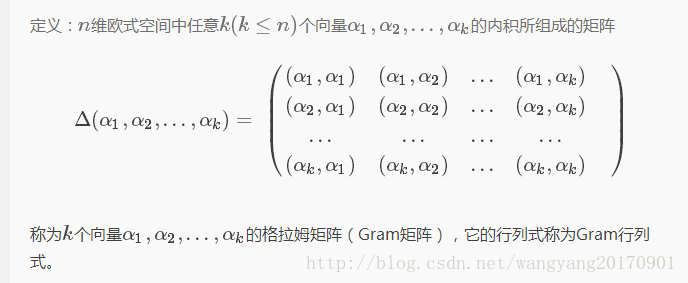
\includegraphics[width=\textwidth]{gram}
\end{document}